\documentclass[12pt,a4paper, margin=3in]{article}
\usepackage[utf8]{inputenc}
\usepackage[margin=.75in]{geometry}
\usepackage{amsmath}
\usepackage{tikz}

\setlength{\parindent}{0em}
\setlength{\parskip}{2em}

\begin{document}

\subsection*{Explain how diodes can be used to non-linearly combine (ie multiply) the input signal and the LO signal in the mixer.} 

\large A diode's I-V characteristic is non-linear. In particular the current \textit{I} through an ideal diode as a function of the voltage \textit{V} across it is given by - \Large \begin{equation} I = I_0 (e^\frac{qV}{   nkT} - 1) \end{equation} 
\large where \textit{q, n, k} are constants and \textit{T} is temperature. The exponential function can be expressed as its Taylor's series. Using $x = \frac{qV}{nkT}$, then the expression in the parenthesis becomes - \Large \begin{equation} e^x - 1 \approx x + \frac{x^2}{2} \end{equation}
\large neglecting higher order terms. Consider V to be composed of two voltages, $V_1$ and $V_2$, the former being one of the frequencies in the RF signal and the other being the LO frequency. The output voltage of the diode can be made proportional to the output current and so the output voltage $V_0$ is (disregarding $I_0$ and the constants in x) - \begin{equation} V_0 \approx (V_1 + V_2) + \frac{(V_1 + V_2)^2}{2} \end{equation} 

The first parenthesis simply gives the 2 input frequencies. Writing $V_1$ as $sin(at)$ and $V_2$ as $sin(bt)$, and expanding the square, the second term becomes - \begin{displaymath} \frac{1}{2}(sin^2(at) + sin^2(bt) + 2 sin(at) sin(bt)) \end{displaymath} 

By trigonometric identity, the cross-product term in this becomes - \begin{displaymath} cos((a - b)t) - cos((a + b)t) \end{displaymath}

So finally, $V_0 = cos((a - b)t) + cos((a + b)t) $ + other frequencies. This is how a diode can be used in a mixer to get signals with down-converted frequencies. The $a - b$ frequency is chosen and the rest are filtered out. Here we took a pair of RF frequency and LO frequency. The LO signal is much stronger than the RF signal. So pairs having 2 RF frequencies will be very small (since their amplitudes are multiplied) so their outputs can be neglected. Only the pairs having one RF frequency and the other one being LO give significant output.  


\subsection*{Quantitatively explain how much improvement in SNR is obtained when the signal is integrated at the integrator. How does the improvement depend on the integration time?}

\large The noise in the signal is assumed to be Gaussian in nature. Noise generated at every instant is independent of other instants and so the noise values at every point are independent random variables. Let the mean of the Gaussian distribution of all these random variables be $\mu$ and the variance be $\sigma^2$. We know from statistics that the mean of \textit{n} such random variables is also a random variable with a Gaussian distribution, with the mean being $\mu$ itself and the variance being $\frac{\sigma^2}{n}$.

Integration of the detected signal can be thought of as this new random variable. After integration the signal's average value is still the average power of the signal after detection. But the average fluctuations in the signal (which is the standard deviation) before and after integration is different. As stated above, the variance gets reduced by a factor of \textit{n}, so the std deviation gets reduced by the factor of $\sqrt{n}$. 

\textit{n} is the number of values that are averaged. The longer the integration time we take, the value of n increases linearly. Also, upon increasing the bandwidth ($\Delta\nu$) of the allowed signal, the number of sampled points directly increases. So the product of $\tau$ and $\Delta\nu$ is proportional to \textit{n}. So the std deviation of the signal value after integration (which is the noise value), is \underline{inversely proportional} to the square-root of the product of $\tau$ and $\Delta\nu$. This noise is also directly proportional to the noise before integration (which is nothing but the std deviation before integration). Denoting the std deviation before and after integration to $\sigma_1$ and $\sigma_2$ - 
\begin{equation} \sigma_2 = \frac{\sigma_1}{\sqrt{\tau \Delta \nu}} \end{equation} 

Hence the SNR increases with the square-root of the integration time. For ex, increasing the integration time by a factor of 4 reduces the noise by factor of 2 which doubles the SNR.

\newpage

\subsection*{To characterize the input and output signal at every stage in the block diagram in terms of amplitude, frequency, phase etc.}

\large The characteristics of the signal at the output of various stages of the processing line are given below-
\begin{itemize}
    \item \underline{Antenna} - The signal has a large range of frequencies limited mainly by the antenna itself. The magnitude of the signal is very small and is accompanied by noise from the astronomical source, sky and man-made sources.
    \item \underline{Pre-amplifier/Amplifier} - The strength (amplitude) of the signal including the pre-existing noise is much increased. The relatives phases between the various frequency components of the signal change because of the linear phase response of the amplifier.
    \item \underline{Mixer} - The signal gets down-converted to a much lower frequency called intermediate frequency (IF). The amplitude drops because power gets distributed to other frequencies apart from IF which are discarded by the mixer. 
    \item \underline{Band-pass filter} - only a smaller range of frequencies remain in the signal and the phase relationships between the frequencies change because filters are also required to have a linear phase response.
\end{itemize}
Until now the signal was AC; the mean of the signal was zero with a non-zero power given by the variance.
\begin{itemize}
    \item \underline{Square-law detector} - now the average value of the signal is non-zero and is equal to the power of the signal. Also the signal gets converted to DC.
    \item \underline{Integrator} - the std deviation of the signal is decreased and its more smoothed out.  
\end{itemize}

\newpage

\subsection*{Explain the folding algorithm of pulsar detection through a flow chart taking into account the subtle and mathematical challenges in the previously given qualitative explanation of folding.}

\large The recorded data which we have to analyse is always discrete in nature. There is some sampling rate at which the changing voltages of the signal are sampled. So we have countably many data points. Lets use a finite length time series with 16 data points only. We represent this time series in the following way - 

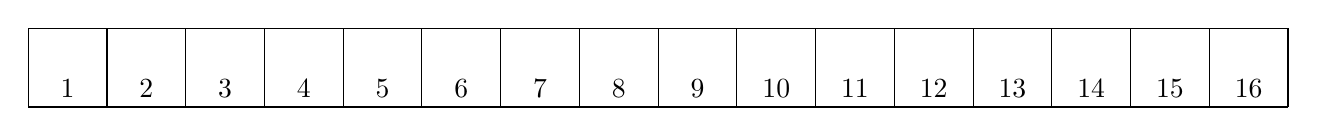
\begin{tikzpicture}
\draw [step=1cm,black,thin] (-8,0) grid (8,1); 

\foreach \x in {1,2,3,4,5,6,7,8,9,10,11,12,13,14,15,16}
   \draw (\x-8.5, 0) node[anchor=south] {$\x$};
\end{tikzpicture}

where each square represents one data point and are numbered in order. This time series is divided into 4 groups and then the values of each group are added to the corresponding values of other groups in the following manner

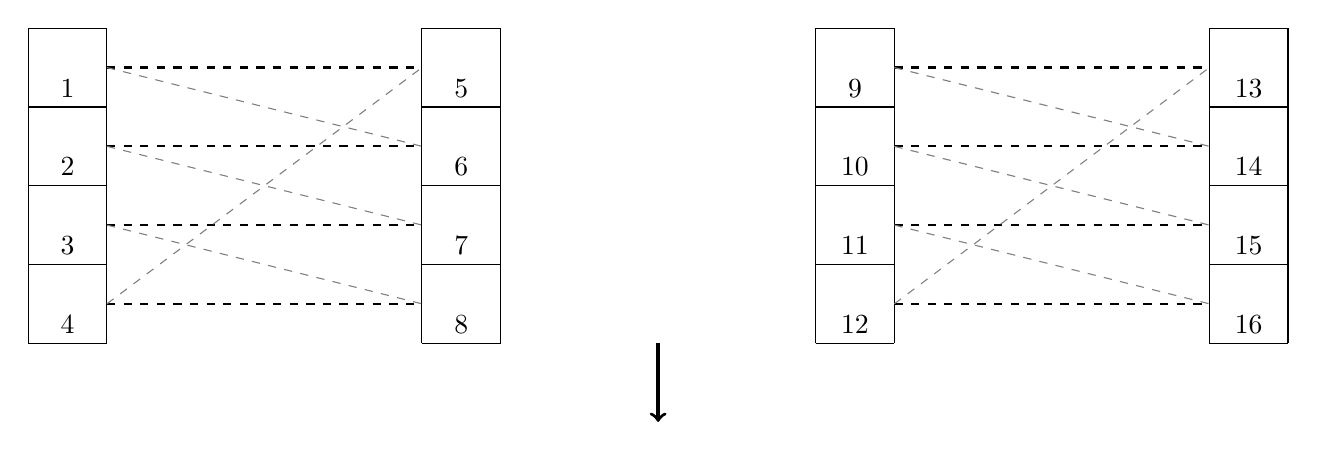
\begin{tikzpicture}

\draw [step=1cm,black,thin] (-7,0) grid (-6,4); 
\foreach \x in {1,2,3,4}
   \draw (-6.5, -\x+4) node[anchor=south] {$\x$};
   
\draw [step=1cm,black,thin] (-2,0) grid (-1,4); 
\foreach \x in {5,6,7,8}
   \draw (-1.5, -\x+8) node[anchor=south] {$\x$};

\draw [step=1cm,black,thin] (3,0) grid (4,4); 
\foreach \x in {9,10,11,12}
   \draw (3.5, -\x+12) node[anchor=south] {$\x$};
   
\draw [step=1cm,black,thin] (8,0) grid (9,4); 
\foreach \x in {13,14,15,16}
   \draw (8.5, -\x+16) node[anchor=south] {$\x$};
   
\draw[dashed,thick] (-6,3.5) - - (-2,3.5);
\draw[dashed,thick] (-6,2.5) - - (-2,2.5);
\draw[dashed,thick] (-6,1.5) - - (-2,1.5);
\draw[dashed,thick] (-6,0.5) - - (-2,0.5);

\draw[dashed,gray] (-6,3.5) - - (-2,2.5);
\draw[dashed,gray] (-6,2.5) - - (-2,1.5);
\draw[dashed,gray] (-6,1.5) - - (-2,.5);
\draw[dashed,gray] (-6,.5) - - (-2,3.5);

\draw[dashed,thick] (4,3.5) - - (8,3.5);
\draw[dashed,thick] (4,2.5) - - (8,2.5);
\draw[dashed,thick] (4,1.5) - - (8,1.5);
\draw[dashed,thick] (4,0.5) - - (8,0.5);

\draw[dashed,gray] (4,3.5) - - (8,2.5);
\draw[dashed,gray] (4,2.5) - - (8,1.5);
\draw[dashed,gray] (4,1.5) - - (8,.5);
\draw[dashed,gray] (4,.5) - - (8,3.5);

\draw[very thick,->] (1,0) -- (1,-1);

\end{tikzpicture}

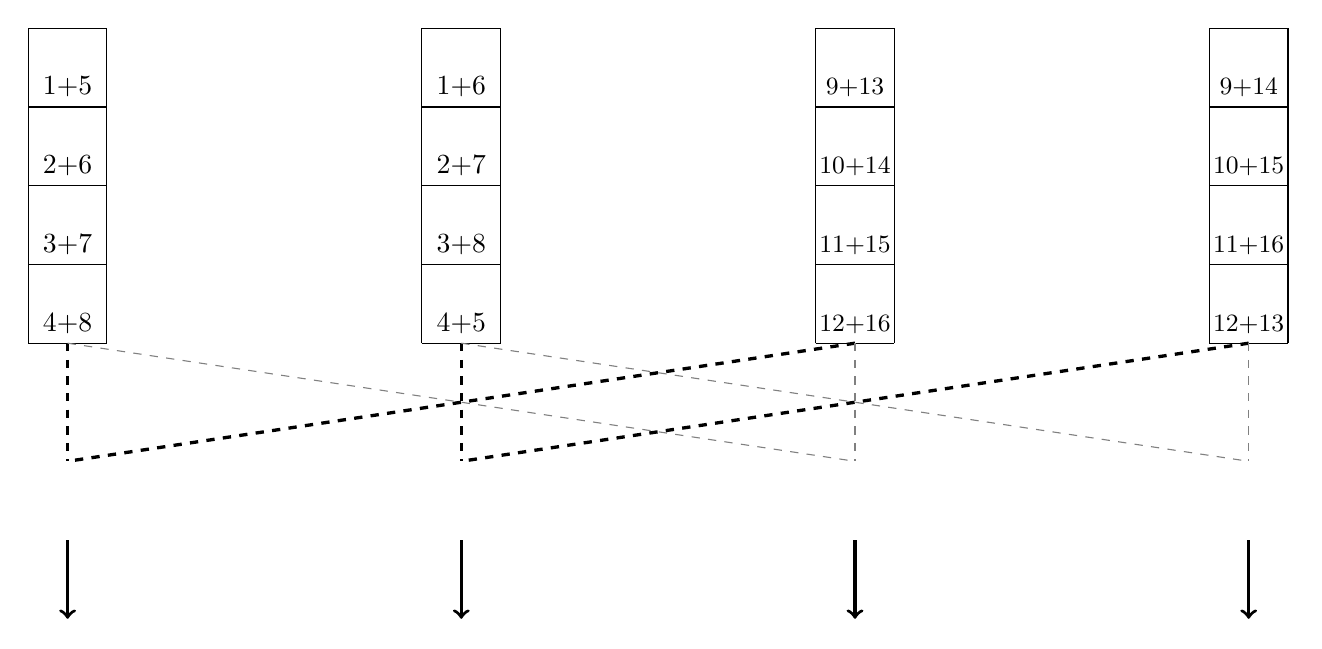
\begin{tikzpicture}

\draw [step=1cm,black,thin] (-7,0) grid (-6,4); 
\draw (-6.5, 3) node[anchor=south] {\normalsize 1+5};
\draw (-6.5, 2) node[anchor=south] {\normalsize 2+6};
\draw (-6.5, 1) node[anchor=south] {\normalsize 3+7};
\draw (-6.5, 0) node[anchor=south] {\normalsize 4+8};
   
\draw [step=1cm,black,thin] (-2,0) grid (-1,4); 
\draw (-1.5, 3) node[anchor=south] {\normalsize 1+6};
\draw (-1.5, 2) node[anchor=south] {\normalsize 2+7};
\draw (-1.5, 1) node[anchor=south] {\normalsize 3+8};
\draw (-1.5, 0) node[anchor=south] {\normalsize 4+5};


\draw [step=1cm,black,thin] (3,0) grid (4,4); 
\draw (3.5, 3) node[anchor=south] {\small 9+13};
\draw (3.5, 2) node[anchor=south] {\small 10+14};
\draw (3.5, 1) node[anchor=south] {\small 11+15};
\draw (3.5, 0) node[anchor=south] {\small 12+16};

   
\draw [step=1cm,black,thin] (8,0) grid (9,4); 
\draw (8.5, 3) node[anchor=south] {\small 9+14};
\draw (8.5, 2) node[anchor=south] {\small 10+15};
\draw (8.5, 1) node[anchor=south] {\small 11+16};
\draw (8.5, 0) node[anchor=south] {\small 12+13};

\draw[dashed,very thick] (-6.5,0) - - (-6.5,-1.5);
\draw[dashed,very thick] (3.5,0) - - (-6.5,-1.5);
\draw[dashed,gray] (3.5,0) - - (3.5,-1.5);
\draw[dashed,gray] (-6.5,0) - - (3.5,-1.5);

\draw[dashed,very thick] (-1.5,0) - - (-1.5,-1.5);
\draw[dashed,very thick] (8.5,0) - - (-1.5,-1.5);
\draw[dashed,gray] (8.5,0) - - (8.5,-1.5);
\draw[dashed,gray] (-1.5,0) - - (8.5,-1.5);

\draw[very thick,->] (-6.5,-2.5) -- (-6.5,-3.5);
\draw[very thick,->] (-1.5,-2.5) -- (-1.5,-3.5);
\draw[very thick,->] (3.5,-2.5) -- (3.5,-3.5);
\draw[very thick,->] (8.5,-2.5) -- (8.5,-3.5);

\end{tikzpicture}

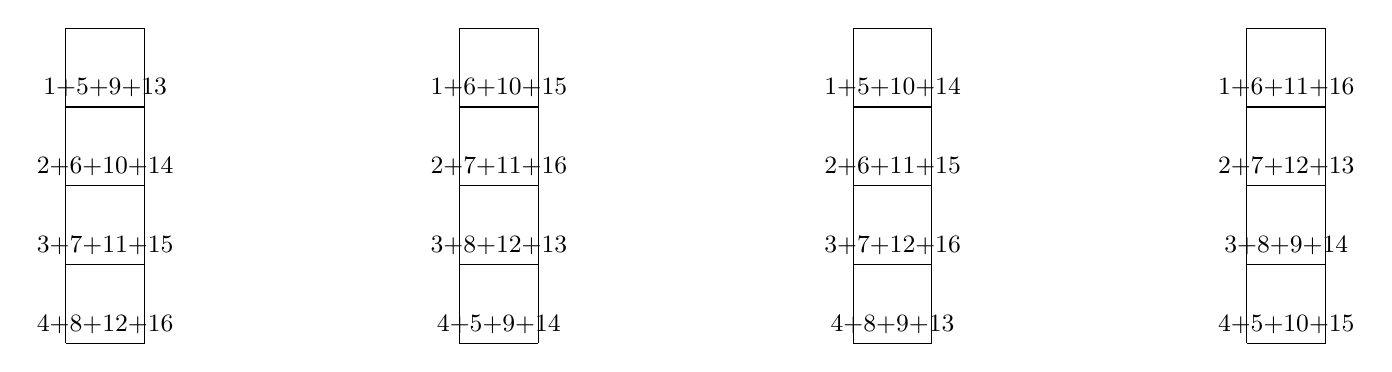
\begin{tikzpicture}

\draw [step=1cm,black,thin] (-7,0) grid (-6,4); 
\draw (-6.5, 3) node[anchor=south] {\small 1+5+9+13};
\draw (-6.5, 2) node[anchor=south] {\small 2+6+10+14};
\draw (-6.5, 1) node[anchor=south] {\small 3+7+11+15};
\draw (-6.5, 0) node[anchor=south] {\small 4+8+12+16};
   

\draw [step=1cm,black,thin] (3,0) grid (4,4); 
\draw (-1.5, 3) node[anchor=south] {\small 1+6+10+15};
\draw (-1.5, 2) node[anchor=south] {\small 2+7+11+16};
\draw (-1.5, 1) node[anchor=south] {\small 3+8+12+13};
\draw (-1.5, 0) node[anchor=south] {\small 4+5+9+14};

\draw [step=1cm,black,thin] (-2,0) grid (-1,4); 
\draw (3.5, 3) node[anchor=south] {\small 1+5+10+14};
\draw (3.5, 2) node[anchor=south] {\small 2+6+11+15};
\draw (3.5, 1) node[anchor=south] {\small 3+7+12+16};
\draw (3.5, 0) node[anchor=south] {\small 4+8+9+13};

\draw [step=1cm,black,thin] (8,0) grid (9,4); 
\draw (8.5, 3) node[anchor=south] {\small 1+6+11+16};
\draw (8.5, 2) node[anchor=south] {\small 2+7+12+13};
\draw (8.5, 1) node[anchor=south] {\small 3+8+9+14};
\draw (8.5, 0) node[anchor=south] {\small 4+5+10+15};

\end{tikzpicture}

Basically in the first step, we add corresponding values of group 1 and 2 in two ways: one is direct overlap and the other is summing after offsetting group 1 by one value ie the first value is paired with the second value of group 2 and so on. Similar thing is done with group 3 and 4. So the first step results in 4 new groups.

In the second step, the new group 1 is paired with the new group 3 again in the same 2 different ways as explained above. Group 2 is paired with group 4 in two ways, one with an offset of 1 value and the other with an offset of 2 values. This again results in 4 new groups which are 4 folded time series with slightly different time periods. In each box in group 1 all values are separated by 4 $t_{sampling}$ (time between 2 consecutive sampling), so group 1 is the folded time series with the period of 4.

Similarly group 2, 3 and 4 are folded time series with period of 14/3, 13/3 and 5 respectively, if we consider the errors due to the sample being discrete to be negligible. Hence with one base period of 4, we got folded time series of 3 other time periods. The schematic shown above can be generalised to time series arbitrarily longer than 16 samples but this schematic works when $log_{2} (\frac{N}{P})$ is an integer, where $N$ is the total number of samples (like 16 in the above example) and $P$ is the base period (like 4 above). 

In this way, folded time series of a large number of periods can be computed. Then the relative merit of each folded time series is determined to find possible pulsar candidates. 

\end{document}